\documentclass[russian]{beamer}  % [t], [c], или [b] --- вертикальное выравнивание на слайдах (верх, центр, низ)
%\documentclass[handout]{beamer} % Раздаточный материал (на слайдах всё сразу)
%\documentclass[aspectratio=169]{beamer} % Соотношение сторон

%\usetheme{Berkeley} % Тема оформления
%\usetheme{Bergen}
%\usetheme{Szeged}

%\usecolortheme{beaver} % Цветовая схема
%\useinnertheme{circles}
%\useinnertheme{rectangles}

\usetheme{Antibes}
\usecolortheme{crane}

%%% Работа с русским языком
\usepackage{cmap}					% поиск в PDF
\usepackage{mathtext} 				% русские буквы в формулах
\usepackage[T2A]{fontenc}			% кодировка
\usepackage[utf8]{inputenc}			% кодировка исходного текста
\usepackage[english,russian]{babel}	% локализация и переносы

%% Beamer по-русски
\newtheorem{rtheorem}{Теорема}
\newtheorem{rproof}{Доказательство}
\newtheorem{rexample}{Пример}

%%% Дополнительная работа с математикой
\usepackage{amsmath,amsfonts,amssymb,amsthm,mathtools} % AMS
\usepackage{icomma} % "Умная" запятая: $0,2$ --- число, $0, 2$ --- перечисление

%% Номера формул
%\mathtoolsset{showonlyrefs=true} % Показывать номера только у тех формул, на которые есть \eqref{} в тексте.
%\usepackage{leqno} % Нумерация формул слева

%% Свои команды
\DeclareMathOperator{\sgn}{\mathop{sgn}}

%% Перенос знаков в формулах (по Львовскому)
\newcommand*{\hm}[1]{#1\nobreak\discretionary{}
	{\hbox{$\mathsurround=0pt #1$}}{}}

%%% Работа с картинками
\usepackage{graphicx}  % Для вставки рисунков
\graphicspath{{images/}{images2/}}  % папки с картинками
\setlength\fboxsep{3pt} % Отступ рамки \fbox{} от рисунка
\setlength\fboxrule{1pt} % Толщина линий рамки \fbox{}
\usepackage{wrapfig} % Обтекание рисунков текстом

%%% Работа с таблицами
\usepackage{array,tabularx,tabulary,booktabs} % Дополнительная работа с таблицами
\usepackage{longtable}  % Длинные таблицы
\usepackage{multirow} % Слияние строк в таблице

%%% Программирование
\usepackage{etoolbox} % логические операторы

%%% Другие пакеты
\usepackage{lastpage} % Узнать, сколько всего страниц в документе.
\usepackage{soul} % Модификаторы начертания
\usepackage{csquotes} % Еще инструменты для ссылок
%\usepackage[style=authoryear,maxcitenames=2,backend=biber,sorting=nty]{biblatex}
\usepackage{multicol} % Несколько колонок

%%% Картинки
\usepackage{tikz} % Работа с графикой
\usepackage{pgfplots}
\usepackage{pgfplotstable}

\title{Праздничный ужин}
%\subtitle{Але-оп}
\author{Иван Иванович Иванов}
\date{\today}

\begin{document}
	\begin{frame}
		\maketitle
	\end{frame}

	\begin{frame}
	\frametitle{Оглавление}
	\tableofcontents
	\end{frame}

	\section{Меню}
	\subsection{Горячие блюда}
	\begin{frame}
		\frametitle{\insertsection} 
		\framesubtitle{\insertsubsection}
		\begin{multicols}{2}
			\begin{itemize}
			\item<1->	Свиная шейка\\
				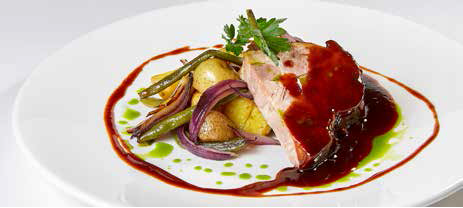
\includegraphics[scale=0.45]{hot_1}
			\item<2->	Стейк из свинины\\
				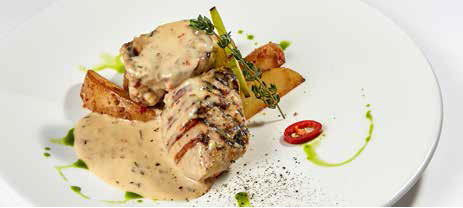
\includegraphics[scale=0.45]{hot_2}
			\item<3->	Каре ягненка\\
				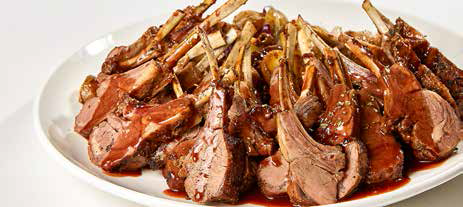
\includegraphics[scale=0.45]{hot_3}
			\item<4->	Филе говядины\\
				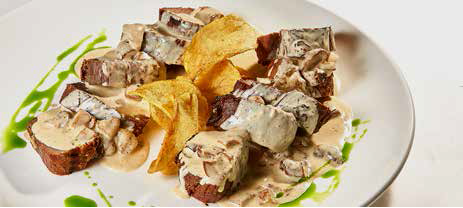
\includegraphics[scale=0.45]{hot_4}
			\end{itemize}
		\end{multicols}
	\end{frame}

	\subsection{Салаты}
	\begin{frame}
		\frametitle{\insertsection} 
		\begin{multicols}{2}
			\begin{itemize}
				\item<1->	Цезарь с курицей\\
				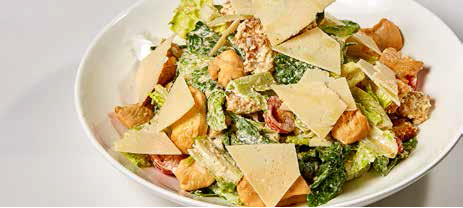
\includegraphics[scale=0.45]{salad_1}
				\item<2->	Швейцарский\\
				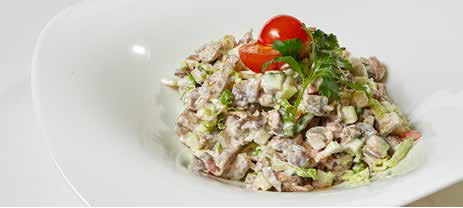
\includegraphics[scale=0.45]{salad_2}
				\item<3-> 	Грибной с языком\\
				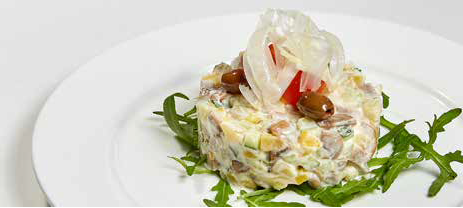
\includegraphics[scale=0.45]{salad_3}
				\item<4-> 	Сельдь под шубой\\
				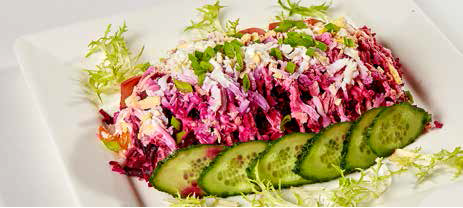
\includegraphics[scale=0.45]{salad_4}
			\end{itemize}
		\end{multicols}
		\framesubtitle{\insertsubsection}
	\end{frame}
	
	\section{Всякие мелочи}
	\begin{frame}
		\frametitle{\insertsection} 
		\begin{block}{Скатерть}
			Можно взять несколько вариантов: либо классический и беспроигрышный вариант "--- белоснежная скатерть, либо однотонными и с рисунком.
		\end{block}
	    \begin{block}{Сервировка}
			Закусочная тарелка ставится на подставочную, с левой стороны – пирожковая. Между ними располагаются столовые приборы — справа нож и ложку, а слева – столовую вилку. А впереди столовые приборы – фужеры.
		\end{block}
		\begin{block}{Источник меню}
			\url{https://www.arti-land.ru/upload/iblock/030/0306f6754860f463f1a0060dd519f344.pdf} 
		\end{block}
	\end{frame}

\end{document}